\documentclass[titlepage,a4paper]{jsarticle}
\usepackage{../../sty/import}%各種パッケージインポート
\usepackage{../../sty/title_team}%タイトルページの変更
% レポートタイトル
\title{球体-木製ブロック衝突実験の\\重回帰分析を用いた分析}
% 提出日
\expdate{\today}
% 科目名
\subject{情報システム工学実験}
% 分野
\class{情報経営システム工学分野}
% 学年
\grade{B3}
% 学籍番号
\mynumber{学籍番号}
% 記述者
\author{本間三暉}
% グループ名
\team{10}
\coauthor{%
{学籍番号:}22100289 & {氏名:}浅野 繭\\
{学籍番号:}22105590 & {氏名:}筒井 翼\\
{学籍番号:}22100986 & {氏名:}板山修大\\
}
\begin{document}
\maketitle
\section{はじめに}
% 本実験の目的や行ったことを記述
\subsection{前置き}
今回の実験で物理実験を行うに当たり,16班に分かれ,各班ごとに実験を行い実験結果をExcelにまとめた.
その実験結果を一つにまとめる際ラベル等の指定がなかったため,おおよそデータの分析を行うとは思えないような形式でまとめている班が散見された.

そのため,各班に呼びかけ形式の統一を行うよう呼びかけた.
しかし,レポート執筆時点(2024年6月27日)で,形式の統一が行われておらずどの数字が実験データかわからない班が3班,単位が正しく直されていなさそうな班が1班いた.

そのような数字はデータの前処理の段階で排除したため,16班分のデータを用いた想定通りのデータ分析が行えないことを断っておきたい.
また,形式を統一した際に,平均値のみを提出した班と生データを提出した班があるため,データの数に偏りがあることも断っておきたい.

\subsection{目的}
現代社会において,データサイエンスの重要性はますます高まっている.
データサイエンスとは,与えられたデータに基づいて知見を見出し,その知見を次の行動に活かすことを目的としている.
本レポートでは,データ分析の基本的な手法とその応用について実験を通じて探求する.

本実験は,データ分析の5つの手順(PPDACサイクル)に基づいて進められる.
PPDACサイクルは,問題の把握(Problem),調査の計画(Plan),データの収集(Data),データの分析(Analysis),および結論の考(Conclusion)
の5つのステップから成り立つ.
これらのステップを踏むことで,データから有用な情報を引き出し,具体的な課題解決に繋げることを目指す.

本レポートの目的は,実験を通じてデータ分析の基本的な手法を理解し,実際のデータを用いた分析のプロセスを経験することである.
さらに,得られた知見をもとに具体的な解決策を提案し,実務に応用できるスキルを身につけることを目指す.

\section{データ(実験概要)}
% どのような実験装置でどういったデータを取ったかを記述
% 他の球体とブロックを使った実験データは,他のグループのデータを採用する.
今回の実験では,図\ref{実験装置}のような装置を用いて行う.
\begin{figure}[H]
  \centering
  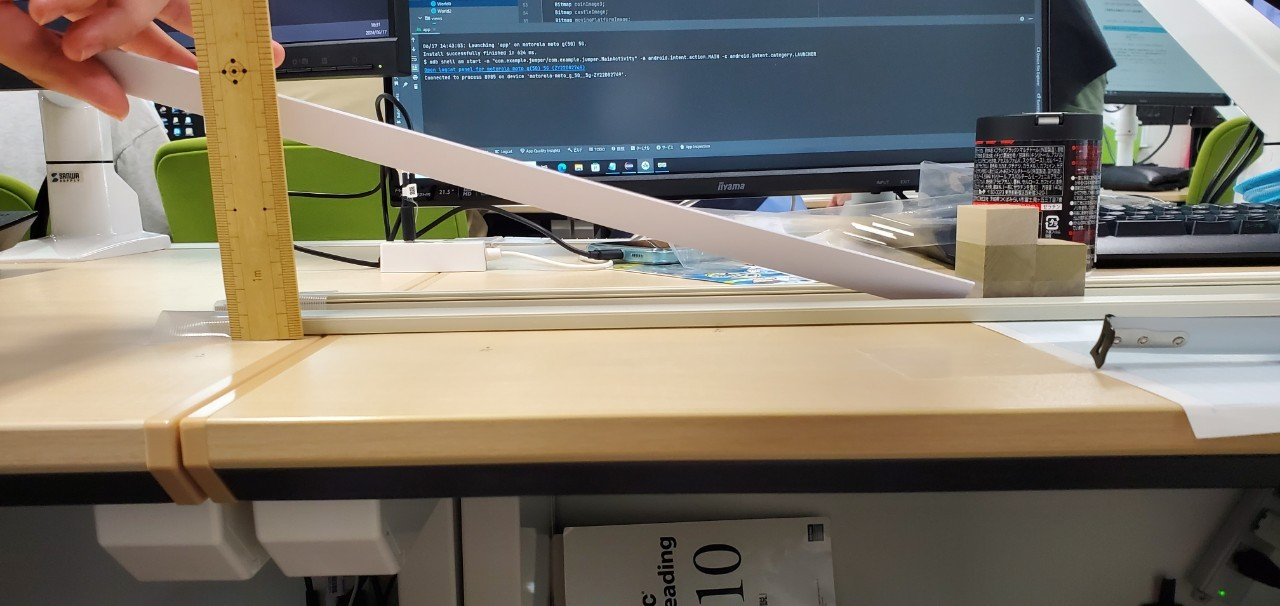
\includegraphics[width=12cm]{img/data_science1.jpg}
  \caption{実験装置}
  \label{実験装置}
\end{figure}

今回,私の班はボールが転がり始める高さ(以下高さ),ボールが転がった距離の内地面と平行な向きに移動した距離(以下底辺),物体の移動距離(以下移動距離)を測定し,
ボールが転がる距離(以下斜辺),斜辺と底辺のなす角(角度)などは計算で導出することにした.
斜辺の導出方法は,斜辺を$C$,高さを$A$,底辺を$B$とした時,三平方の定理から式\eqref{Pythagoras}で導出できる.
\begin{align}
  C^{2} & = A^{2} + B^{2}                           \\
  C     & = \sqrt{A^{2} + B^{2}} \label{Pythagoras}
\end{align}

また,角度は測定値である高さと底辺から導出する.
高さを$A$,底辺を$B$,角度を$\theta$とした時,タンジェントの定義式から,アークタンジェントを用いた式\eqref{atan}から導出できる.
\begin{align}
  \tan \theta & = \frac{A}{B}                                   \\
  \theta      & = \arctan \left(\frac{A}{B}\right) \label{atan}
\end{align}

Excelの関数ATAN()は戻り値の単位がラジアンなので,これを度数法に直す必要がある.
弧度法は,扇形を考えた時,中心角$\theta$は円弧の長さ$l$に比例する.
円弧の長さ$l$と扇型の半径$r$の比をとると,同じ角度$\theta$に対して扇型の大きさにかかわらずこの比は一定である.
このような性質を利用して,角度の大きさは式\eqref{rad}を用いて定義されている.
\begin{align}
  \theta & = \frac{l}{r}\label{rad}
\end{align}

よって弧度法から度数法に変換するためには,弧度法の角度を$\theta$,度数法の角度を$\theta'$とした時,式\eqref{convert}を用いれば良い.
\begin{align}
  \theta' & = \frac{360}{2\pi}\theta \label{convert}
\end{align}

また,今回は情報経営システム工学分野B3の学生を4人で1つの班に分け,全部で16班作成する.
各班ごとに使用するボールの重さや材質,物体の重さを変え実験を行う.
ボールの種類は以下の7種類である.
\begin{itemize}
  \item 鉄球1
  \item 鉄球2
  \item 鉄球3
  \item ビー玉1
  \item ビー玉2
  \item スーパーボール
  \item ゴムボール
\end{itemize}
また,物体の重さは5段階である.

私の班は重さが$66.9[g]$の鉄球をボールに用いて,重さが$25.7[g]$で地面との接地面積が$1350[mm^{2}]$の物体を用いて実験を行った.


\section{データの前処理}
% 前処理で行ったことを記述
\subsection{データの前処理について}
データの前処理は,データ分析工程の8割を占めるとも言われるほど重要な工程である.
必要な情報が完璧にそろっているデータは珍しく,多くのデータは必要な数値が抜けている場合がほとんどである.
さらに,データごとに形式が違うこともあり,数値に変換されていないテキストデータ(文字データ)しかない場合も多々ある.
このような状態のデータではエラーが発生しやすく,不十分な結果しか得られないため,データの前処理を行って事前にデータを整理する必要がある.
データの形式や質・量が予測精度を決定するため,前処理はスムーズに分析を行うために不可欠であり,予測精度を担保するための重要な開発工程である.

データの前処理には大きく分けて5つの方法がある.
\subsubsection{数値型への変換}
本来数値型が入力されるべき場所に文字列や記号が入力されている場合がある.
例えば,Excelのデータで他の欄には数値データが入っているにもかかわらず,一箇所に「測定不可」のようなメモが残されている場合がある.
そのような文字列データを除去し,全てのデータを数値型に置き換える必要がある.

\subsubsection{欠損値処理}
欠損値とは,何らかの理由により記載されなかったり欠落したりした値のことである.欠損値の対処法としては以下の方法がある.
\begin{itemize}
  \item 平均値や最頻値で補完する:欠損値を含むデータが分析に必要な場合は,平均値や最頻値で補完する.
        欠損値を含むデータを全て除外するとデータ数が不足する場合などは,できる限り補完を検討する.
  \item 行または列ごと除外する:欠損値の割合が高い行や列がある場合は,そのデータを分析対象から除外する.
\end{itemize}
\subsubsection{外れ値処理}
ヒストグラムや散布図を用いてデータの分布を確認し,外れ値の有無を確認する.外れ値の対処法としては以下のようなものがある.
\begin{itemize}
  \item 正しい値に修正する:外れ値がデータの入力ミスやシステムのエラーによる場合は,正しい値に修正する.
  \item 行ごと除外する:外れ値が分析結果に大きな影響を与える場合は,行ごと除外する.
  \item そのまま使用する:外れ値が分析結果に影響しない場合は,そのまま使用することもある.
\end{itemize}
\subsubsection{スケーリング}
データの値を特定の範囲に変換する前処理方法である.
例えば,異なる単位のデータを比較する際に単位をそろえたり,データの値を同じスケールにそろえたりするためによく使われるスケーリングの手法には,
「Min-Maxスケーリング」や「Zスコアスケーリング」などがある.
\begin{itemize}
  \item Min-Maxスケーリングはデータを最小値0,最大値1にスケーリングする方法である.
  \item Zスコアスケーリングは平均0,分散1にスケーリングする方法で,大きな外れ値がある場合に適している.
  \item Robustスケーリングは,データの中央値を0,四分位範囲を1として変換する手法で,外れ値の影響を受けにくい.
\end{itemize}
\subsubsection{ダミーデータ}
ダミー変数の作成がある.質的データやカテゴリカルデータを数字に変換する手法であり,例えばカテゴリを「0」と「1」に変換する方法がある.
例えば,「はい」を1,「いいえ」を0にしたり,「男」を1,「女」を0に変換する.
3つ以上のカテゴリがある場合は,各カテゴリを1とし,その他を0とした数列に変換する.
\subsection{グループデータ}
% ・グループデータ
実験時にデータを取得した際,高さ$200[mm]$,底辺$100[mm]$のときボールが物体を弾いてしまい上手くデータが取れなかったため,"N/A"と記述した.
しかし,データ分析の際にはそのようなデータは不要なため行ごと削除した.
\subsection{統合データ}\label{外れ血}
% ・全グループ統合データ
実験時各班でデータを作成したため,フォーマットや基準にする単位がバラバラになってしまっていた.
それだけならいいが,表を横に作成する班,シートを増やしすぎている上に名前を変えずそもそもデータがどこにあるか分かりにくい班,
単位を明記していない班など様々であった.

そのため,各班ごとにフォーマットとデータの単位を表\ref{テンプレ}のような形に整形するよう呼びかけた.また,表が横に長いため途中で折り返して示す.
\begin{table}[H]
  \centering
  \caption{整形後フォーマット}
  \label{テンプレ}
  \begin{tabular}{lllll}
    移動距離{[}mm{]}    & 底辺{[}mm{]}                       & 高さ{[}mm{]}                       & 斜辺{[}mm{]} & 理論値角度{[}度{]}                      \\\hline\hline
    20              & 430                              & 100                              & 441.475    & 13.092                            \\\hline
    理論値角度{[}ラジアン{]} & \multicolumn{1}{r}{球体の質量{[}g{]}} & \multicolumn{1}{r}{物体の質量{[}g{]}} & 球体の種類      & 物体の底面積{[}mm\textasciicircum{}2{]} \\\hline\hline
    0.228           & 5.5                              & 10.5                             & 鉄球1        & 1305                              \\\hline
  \end{tabular}
\end{table}

呼びかけの結果,多くの班でデータのフォーマットが統一された.
フォーマットを統一してくれず基準にした単位も記述されていないような修正のしようがない班のデータは除外した.
また,ボールの素材によって別の分析をする必要があったのでダミー変数を追加した.
ダミー変数を追加する際,式\eqref{excel}に示すExcel関数を用いて作成した.
\begin{align}
  =IF(MID(\$I2,1,1)="鉄",1,0) \label{excel}
\end{align}

ここで,セル$I2$は球体の種類の列の値である.
この式は球体の種類の列を参照し,1文字目が"鉄"であったら1,そうでなかったら0を入力する関数である.
各グループの実験で用いたボールがどの素材であるかは1文字目を参照し,ダミー変数を1にしたい材質の1文字目と比べれば良い.

このようにして表\ref{テンプレ}の右に追加したダミー変数を表\ref{ダミー}に示す.
\begin{table}[H]
  \centering
  \caption{ダミー変数追加}
  \label{ダミー}
  \begin{tabular}{llll}
    鉄球 & ビー玉 & ゴムボール & スーパーボール \\\hline\hline
    1  & 0   & 0     & 0       \\\hline
  \end{tabular}
\end{table}

このように処理したデータを用いて分析を行う.


\section{相関分析・単回帰分析}\label{相関:節}
私のグループで取ったデータに関して相関分析と単回帰分析を行う.
\subsection{相関分析}
相関分析とは,2つの変数間の関係性を定量的に評価する統計手法である.
この分析手法は,様々な分野で広く活用されており,データに隠れた関係性を発見し,因果関係の手がかりを得るために重要な役割を果たしている.

相関分析では,2つの変数間の関係の強さと方向を相関係数によって表現する.
相関係数は-1から1の間の値を取り,1に近いほど正の相関が強く,-1に近いほど負の相関が強いことを示す.
0に近い値は,相関がほとんどない,または全くないことを意味する.

相関分析を行う際には,まず散布図を作成して変数間の関係を視覚的に確認することが重要である.
散布図から関係のパターン(線形,非線形など)を把握した上で,相関係数を計算し,その値に基づいて相関の強さを解釈する.

ただし,相関分析の結果を解釈する際には,いくつかの注意点がある.
相関があることは因果関係を意味するわけではなく,第三の要因が両方の変数に影響を与えている可能性もある.
また,相関係数は外れ値に敏感であるため,データの前処理で外れ値の処理が重要となる.
さらに,Pearsonの相関係数は線形関係を前提としているため,非線形の関係がある場合には他の方法を検討する必要がある.

具体的なデータセットに対して相関分析を適用する際は,データの特性に応じた前処理が必要となる.
例えば,カテゴリカルデータを数値に変換するためにダミー変数を使用したり,変数のスケールを揃えるために標準化を行ったりする.
このように,相関分析は変数間の関係性を理解するための強力なツールであり,適切に使用することで,データから有益な知見を得ることができる.
しかし,分析結果の解釈には注意が必要であり,常に因果関係の可能性を念頭に置きながら,多角的な視点でデータを見ることが重要である.

この実験ではExcelの機能を用いて相関分析を行う.
相関分析を行った結果について表\ref{相関分析}に示す.
\begin{table}[H]
  \caption{相関分析}
  \label{相関分析}
  \begin{tabular}{r|lllll}
                 & \multicolumn{1}{c}{移動距離{[}mm{]}} & \multicolumn{1}{c}{底辺{[}mm{]}} & \multicolumn{1}{c}{高さ{[}mm{]}} & \multicolumn{1}{c}{斜辺{[}mm{]}} & \multicolumn{1}{c}{理論値角度{[}度{]}} \\\hline\hline
    移動距離{[}mm{]} & 1                                &                                &                                &                                &                                  \\
    底辺{[}mm{]}   & 0.456861417                      & 1                              &                                &                                &                                  \\
    高さ{[}mm{]}   & 0.898531378                      & 0.136363636                    & 1                              &                                &                                  \\
    斜辺{[}mm{]}   & 0.616331666                      & 0.972160283                    & 0.352605016                    & 1                              &                                  \\
    理論値角度{[}度{]} & 0.25097754                       & -0.66280947                    & 0.589354047                    & -0.476740815                   & 1                                \\\hline
  \end{tabular}
\end{table}
表\ref{相関分析}から移動距離と強い正の相関があるのは高さであることがわかる.
よって単回帰分析は移動距離と高さで行う.


\subsection{単回帰分析}
%  ・説明変数に「高さ」を選んだ理由
%  ・P値に関して
%  ・決定係数に関して
%  ・相関係数に関して
単回帰分析は,一つの説明変数と目的変数の関係を調べるための統計的手法である.
この分析手法は,説明変数の値から目的変数の値を予測するためのモデルを構築することを目的としている.

単回帰分析を実施するには,まず説明変数と目的変数のデータを収集し,それらの関係を散布図で視覚化する.
散布図から,両変数の間に直線的な関係が存在するかどうかを判断する.
次に,最小二乗法を用いて回帰式の係数を推定する.
この回帰式は,説明変数の値から目的変数の値を予測するために使用される.

推定された回帰式の精度を評価するために,決定係数$R^{2}$を確認する.
$R^{2}$は,回帰式がデータの変動をどの程度説明できるかを示す指標である.
$R^{2}$の値が高いほど,回帰式の当てはまりが良いことを意味する.
また,回帰式の統計的有意性を確認するために,F検定やt検定を行う.

回帰式の係数が統計的に有意であれば,説明変数が目的変数に対して有意な影響を与えていると判断できる.
この場合,説明変数の値を変化させることで,目的変数の値を制御できる可能性がある.

強い正の相関がある移動距離と高さについて単回帰分析を行った結果を表\ref{単回帰分析}に示す.
\begin{table}[H]
  \centering
  \caption{単回帰分析($Y$=移動距離,$X=$高さ)}
  \label{単回帰分析}
  \begin{minipage}[c]{1\hsize}
    \centering
    \subcaption{回帰統計}
    \label{単回帰統計}
    \begin{tabular}{l|l}
      \multicolumn{2}{c}{回帰統計} \\\hline\hline
      重相関 R  & 0.89853138      \\
      重決定 R2 & 0.80735864      \\
      補正 R2  & 0.80471971      \\
      標準誤差   & 91.1275435      \\
      観測数    & 75              \\\hline
    \end{tabular}
  \end{minipage}

  \begin{minipage}[c]{1\hsize}
    \centering
    \subcaption{分散分析表1}
    \label{sub分散1}
    \begin{tabular}{l|lllll}
      \multicolumn{1}{c|}{} & \multicolumn{1}{c}{自由度} & \multicolumn{1}{c}{変動} & \multicolumn{1}{c}{分散} & \multicolumn{1}{c}{観測された分散比} & \multicolumn{1}{c}{有意 F} \\\hline\hline
      回帰                    & 1                       & 2540616.66             & 2540616.66             & 305.942502                   & 8.0769E-28               \\
      残差                    & 73                      & 606208.73              & 8304.22918             &                              &                          \\
      合計                    & 74                      & 3146825.39             &                        &                              &                          \\\hline
    \end{tabular}
  \end{minipage}

  \begin{minipage}[c]{1\hsize}
    \centering
    \subcaption{分散分析表2}
    \label{sub分散2}
    \begin{tabular}{l|llllllll}
      \multicolumn{1}{c|}{} & \multicolumn{1}{c}{係数} & \multicolumn{1}{c}{標準誤差} & \multicolumn{1}{c}{t値} & \multicolumn{1}{c}{P-値} & \multicolumn{1}{c}{下限 95.0\%} & \multicolumn{1}{c}{上限 95.0\%} \\\hline\hline
      切片                    & 23.0606061             & 25.5787529               & 0.90155318             & 0.37025921              & -27.917775                    & 74.0389872                    \\
      高さ{[}mm{]}            & 3.39827273             & 0.19428458               & 17.4912121             & 8.0769E-28              & 3.01106413                    & 3.78548133                    \\\hline
    \end{tabular}
  \end{minipage}
\end{table}

単回帰分析の結果は目的変数を$y$,切片を$\beta_{0}$,回帰係数を$\beta_{1}$,説明変数を$x$としたとき,回帰式は式\eqref{回帰式}のようになる.
\begin{align}
  y    & = \beta_{0} + \beta_{1} \times x         \\
  移動距離 & = 23.0660 + 3.3983 \times 高さ \label{回帰式}
\end{align}

表\ref{単回帰分析}を見ると,決定係数$R^{2}$の値が大きいのでこのモデルにはかなりの説得力がある.
表\ref{sub分散1}の有意 Fは0.01以下の値となっていることから統計的に有意である,この回帰モデルには十分な意味があると解釈できる。
また,表\ref{sub分散2}からP-値を確認すると0.01以下の値となっていることから,高さと移動距離には関係があると考えられる.
同様に,t値の絶対値が17を超えることから,高さは移動距離にとても影響する事がわかる.

\section{重回帰分析}%%% あとで移動距離が平均値の場合についてもやって比較やりたい.あとVIFからの多重共線性も示せたら示したい.
重回帰分析とは,複数の説明変数を用いて一つの目的変数を予測するための統計手法である.
この手法を用いることで,目的変数と複数の説明変数の間の関係をモデル化し,予測精度を向上させることができる.

モデルの構築をする際,重回帰分析に使用する説明変数を慎重に選ぶ必要がある.
多重共線性を避けるために,相関が高い説明変数は同時に使用しないように注意する必要がある.
そして,目的変数と説明変数の関係を表す回帰式を作成する.

モデルを構築した後はその評価を行う.
まず,補正$R^{2}$の値を確認し,モデルの精度を評価する.
この値は0から1の範囲で,1に近いほど高い精度を示す.
また,有意Fの値を確認し,回帰式が統計的に有意かどうかを判断する.
有意Fが0.05未満であれば,有用な回帰式とされる.
さらに,各説明変数のP値を確認し,これが0.05未満であれば,その説明変数は目的変数に対して統計的に有意であると判断する.

結果の解釈も重要である.
各説明変数のt値を確認し,その影響度を評価する.
t値が2より大きい場合,その説明変数は目的変数に対して影響があるとされる.
また,回帰係数の符号と大きさを確認し,目的変数への影響を解釈する.

このような手順で重回帰分析を用いることで複数の要因が目的変数にどのように影響するかを明らかにし,より精度の高い予測を行うことが可能となる.

私のグループで行った実験のデータを用いて重回帰分析した結果を\ref{グループデータ}節に,
全グループのデータを統合し\ref{外れ血}節の処理を行ったデータに対して重回帰分析した結果を\ref{全グループデータ}節に示す.
\subsection{グループデータ}\label{グループデータ}
% ・球体・ブロック各1種のグループデータで行った重回帰分析について記述
%  説明変数の選択方法
%  重回帰式
%  修正済決定係数とあてはまりのよさを記述
% P 値と説明力について記述
% ※余裕があれば未計測の説明変数値での計算予測値と実測値の比較をしてみる
目標変数は移動距離とし,説明変数として高さと底辺を用いる.
1つ目の説明変数である高さは,表\ref{相関分析}を見ると目標変数との相関係数が最も大きいからであり,
2つ目の説明変数は高さと斜辺についで相関が大きいため底辺を用いた.
高さについで相関が大きい斜辺を用いなかった理由は,
式\eqref{Pythagoras}に示すように斜辺の導出に高さを用いてしまっていることと高さと斜辺の相関係数が$0.972160283$とかなり高いことから,
多重共線性が疑われるためである.

目標変数を移動距離,説明変数を高さと底辺として行った重回帰分析の結果を表\ref{重回帰分析1}に示す.
\begin{table}[H]
  \centering
  \caption{グループ重回帰分析($Y$=移動距離,$X_{1}=$高さ,$X_{2}=$底辺)}
  \label{重回帰分析1}
  \begin{minipage}[c]{0.5\hsize}
    \centering
    \subcaption{回帰統計}
    \label{sub1回帰統計}
    \begin{tabular}{l|l}
      \multicolumn{2}{c}{回帰統計} \\\hline\hline
      重相関 R  & 0.95982085      \\
      重決定 R2 & 0.92125606      \\
      補正 R2  & 0.91906873      \\
      標準誤差   & 58.6649407      \\
      観測数    & 75              \\\hline
    \end{tabular}
  \end{minipage}
  \begin{minipage}[c]{1\hsize}
    \centering
    \subcaption{分散分析表1}
    \label{sub1分析}
    \begin{tabular}{l|lllll}
      \multicolumn{1}{c|}{} & \multicolumn{1}{c}{自由度} & \multicolumn{1}{c}{変動} & \multicolumn{1}{c}{分散} & \multicolumn{1}{c}{観測された分散比} & \multicolumn{1}{c}{有意 F} \\\hline\hline
      回帰                    & 2                       & 2899031.97             & 1449515.98             & 421.178057                   & 1.8358E-40               \\
      残差                    & 72                      & 247793.419             & 3441.57527             &                              &                          \\
      合計                    & 74                      & 3146825.39             &                        &                              &                          \\\hline
    \end{tabular}
  \end{minipage}
  \begin{minipage}[c]{1\hsize}
    \centering
    \subcaption{分散分析表2}
    \label{sub2分析}
    \begin{tabular}{l|llllll}
      \multicolumn{1}{c|}{} & \multicolumn{1}{c}{係数} & \multicolumn{1}{c}{標準誤差} & \multicolumn{1}{c}{t値} & \multicolumn{1}{c}{P-値} & \multicolumn{1}{c}{下限 95\%} & \multicolumn{1}{c}{上限 95\%} \\\hline\hline
      切片                    & -123.35088             & 21.8401066               & -5.6479064             & 3.0324E-07              & -166.88833                  & -79.81342                   \\
      高さ{[}mm{]}            & 3.22257895             & 0.12625343               & 25.5246852             & 8.2767E-38              & 2.97089734                  & 3.47426055                  \\
      底辺{[}mm{]}            & 0.64421053             & 0.06312671               & 10.2050383             & 1.2438E-15              & 0.51836972                  & 0.77005133                  \\\hline
    \end{tabular}
  \end{minipage}
\end{table}

重回帰分析の結果は目的変数を$y$,切片を$\beta_{0}$,回帰係数を$\beta_{1}$,$\beta_{2}$,説明変数を$x_{1}$,$x_{2}$としたとき,回帰式は式\eqref{重回帰式1}のようになる.
\begin{align}
  y    & = \beta_{0}+\sum_{k=1}^{n}\left(\beta_{k} \times x_{k}\right)            \\
  移動距離 & = -123.35088 + 3.22257895  \times 高さ+ 0.64421053 \times 底辺 \label{重回帰式1}
\end{align}

表\ref{sub1回帰統計}を見ると,決定係数$R^{2}$の値が大きいのでこのモデルにはかなりの説得力がある.
表\ref{sub1分析}の有意 Fは0.01以下の値となっていることから統計的に有意であり,この回帰モデルには十分な意味があると解釈できる.
また,表\ref{sub2分析}からP-値を確認すると高さと底辺が共に0.01以下の値となっていることから,高さ底辺,移動距離には関係があると考えられる.
同様に,t値の絶対値がそれぞれ25と10を超えることから,高さは移動距離にとても影響し,高さほどでないにしろ底辺も移動距離に影響を与えることがわかる.

\subsection{全グループデータ}\label{全グループデータ}
% ・全グループデータを合わせた重回帰分析について記述
%  説明変数の選択方法
%  重回帰式
%  修正済決定係数とあてはまりのよさを記述
% P 値と説明力について記述
% ※余裕があれば未計測の組み合わせ等での計算予測値と実測値の比較をしてみる
統合データにした場合の相関関係を表\ref{統合相関関係}に示す.
\begin{table}[H]
  \centering
  \caption{統合データ相関関係}
  \label{統合相関関係}
  % tabler環境の挿入
  \begin{tabular}{l|lllllllll}
    \multicolumn{1}{c}{} & \multicolumn{1}{c}{移動距離{[}mm{]}} & \multicolumn{1}{c}{底辺{[}mm{]}} & \multicolumn{1}{c}{高さ{[}mm{]}} & \multicolumn{1}{c}{球体の質量{[}g{]}} & \multicolumn{1}{c}{物体の質量{[}g{]}} \\\hline\hline
    移動距離{[}mm{]}         & 1                                &                                &                                &                                  &                                  \\
    底辺{[}mm{]}           & 0.39095788                       & 1                              &                                &                                  &                                  \\
    高さ{[}mm{]}           & 0.72340443                       & 0.32078803                     & 1                              &                                  &                                  \\
    球体質量{[}g{]}          & 0.3293878                        & -0.2341462                     & -0.089133                      & 1                                &                                  \\
    物体質量{[}g{]}          & 0.45524163                       & -0.1558678                     & -0.0051561                     & 0.87277069                       & 1                                \\
    物体底面積{[}$mm^{2}${]}  & 0.50522081                       & 0.04615244                     & 0.1990338                      & 0.58904821                       & 0.8142857                        \\\hline
  \end{tabular}
\end{table}

\ref{グループデータ}節と同様に目標変数は移動距離とし,説明変数として高さと底辺を用いてサンプル数や違う条件のデータが増えた場合について比較する.

目標変数を移動距離,説明変数を高さと底辺として行った重回帰分析の結果を表\ref{統合重回帰分析0}に示す.

\begin{table}[H]% 最小データ
  \centering
  \caption{統合データ重回帰分析($Y$=移動距離,$X_{1}=$高さ,$X_{2}=$底辺)}
  \label{統合重回帰分析0}
  \begin{minipage}[c]{0.5\hsize}
    \centering
    \subcaption{回帰統計}
    \label{sub1統合回帰統計0}
    \begin{tabular}{l|l}
      \multicolumn{2}{c}{回帰統計} \\\hline\hline
      重相関 R  & 0.73864805      \\
      重決定 R2 & 0.54560094      \\
      補正 R2  & 0.54410128      \\
      標準誤差   & 212.635236      \\
      観測数    & 609             \\\hline
    \end{tabular}
  \end{minipage}
  \begin{minipage}[c]{1\hsize}
    \centering
    \subcaption{分散分析表1}
    \label{sub1統合分析0}
    \begin{tabular}{l|lllll}
      \multicolumn{1}{c|}{} & \multicolumn{1}{c}{自由度} & \multicolumn{1}{c}{変動} & \multicolumn{1}{c}{分散} & \multicolumn{1}{c}{観測された分散比} & \multicolumn{1}{c}{有意 F} \\\hline\hline
      回帰                    & 2                       & 32898854.7             & 16449427.4             & 363.814763                   & 1.598E-104               \\
      残差                    & 606                     & 27399528.5             & 45213.7434             &                              &                          \\
      合計                    & 608                     & 60298383.3             &                        &                              &                          \\\hline
    \end{tabular}
  \end{minipage}
  \begin{minipage}[c]{1\hsize}
    \centering
    \subcaption{分散分析表2}
    \label{sub2統合分析0}
    \begin{tabular}{l|llllll}
      \multicolumn{1}{c|}{} & \multicolumn{1}{c}{係数} & \multicolumn{1}{c}{標準誤差} & \multicolumn{1}{c}{t値} & \multicolumn{1}{c}{P-値} & \multicolumn{1}{c}{下限 95\%} & \multicolumn{1}{c}{上限 95\%} \\\hline\hline
      切片                    & 2.94835813             & 18.1084732               & 0.16281649             & 0.8707172               & -32.614625                  & 38.511341                   \\
      高さ[mm]                & 1.57078417             & 0.0674052                & 23.3036058             & 3.0065E-86              & 1.43840802                  & 1.70316031                  \\
      底辺[mm]                & 0.26200524             & 0.03855161               & 6.79622092             & 2.5742E-11              & 0.18629426                  & 0.33771621                  \\\hline
    \end{tabular}
  \end{minipage}
\end{table}

重回帰分析の結果は目的変数を$y$,切片を$\beta_{0}$,回帰係数を$\beta_{1}$,$\beta_{2}$,説明変数を$x_{1}$,$x_{2}$としたとき,回帰式は式\eqref{統合重回帰式0}のようになる.
\begin{align}
  y    & = \beta_{0}+\sum_{k=1}^{n}\left(\beta_{k} \times x_{k}\right)              \\
  移動距離 & = 2.94835813 + 1.57078417  \times 高さ+ 0.26200524 \times 底辺 \label{統合重回帰式0}
\end{align}

表\ref{sub1統合回帰統計0}を見ると,決定係数$R^{2}$の値は中程度なので,このモデルの説得力は中程度である.
表\ref{sub1統合分析0}の有意 Fは0.01以下の値となっていることから統計的に有意であり,この回帰モデルには十分な意味があると解釈できる.
また,表\ref{sub2統合分析0}からP-値を確認すると高さと底辺が共に0.01以下の値となっていることから,高さ底辺,移動距離には関係があると考えられる.
同様に,t値の絶対値がそれぞれ23と6を超えることから,高さは移動距離にとても影響し,高さほどでないにしろ底辺も移動距離に影響を与えることがわかる.

同じ条件下ではグループデータのみを用いた場合より統合データを用いた場合の精度が下がることがわかった.
そこで,各班ごとの違う条件を反映するため,表\ref{統合相関関係}より高さや底辺との相関係数が低く,多重共線性が起こりにくいであろう球体の重さを用いて重回帰分析を行う.
説明変数を高さと底辺,球体の重さとして行った重回帰分析の結果を表\ref{統合重回帰分析1}に示す.
\begin{table}[H]%球体の重さについて
  \centering
  \caption{統合データ重回帰分析($Y$=移動距離,$X_{1}=$高さ,$X_{2}=$底辺,$X_{3}=$球体の重さ)}
  \label{統合重回帰分析1}
  \begin{minipage}[c]{0.5\hsize}
    \centering
    \subcaption{回帰統計}
    \label{sub統合回帰統計1}
    \begin{tabular}{l|l}
      \multicolumn{2}{c}{回帰統計} \\\hline\hline
      重相関 R  & 0.91281551      \\
      重決定 R2 & 0.83323215      \\
      補正 R2  & 0.8324052       \\
      標準誤差   & 128.720858      \\
      観測数    & 609             \\\hline
    \end{tabular}
  \end{minipage}
  \begin{minipage}[c]{1\hsize}
    \centering
    \subcaption{分散分析表1}
    \label{sub1統合分析1}
    \begin{tabular}{l|lllll}
      \multicolumn{1}{c|}{} & \multicolumn{1}{c}{自由度} & \multicolumn{1}{c}{変動} & \multicolumn{1}{c}{分散} & \multicolumn{1}{c}{観測された分散比} & \multicolumn{1}{c}{有意 F} \\\hline\hline
      回帰                    & 3                       & 50084910.9             & 16694970.3             & 1007.59917                   & 8.767E-235               \\
      残差                    & 605                     & 10024280.9             & 16569.0593             &                              &                          \\
      合計                    & 608                     & 60109191.8             &                        &                              &                          \\\hline
    \end{tabular}
  \end{minipage}
  \begin{minipage}[c]{1\hsize}
    \centering
    \subcaption{分散分析表2}
    \label{sub2統合分析1}
    \begin{tabular}{l|llllll}
      \multicolumn{1}{c|}{} & \multicolumn{1}{c}{係数} & \multicolumn{1}{c}{標準誤差} & \multicolumn{1}{c}{t値} & \multicolumn{1}{c}{P-値} & \multicolumn{1}{c}{下限 95\%} & \multicolumn{1}{c}{上限 95\%} \\\hline\hline
      切片                    & -243.03891             & 14.472797                & -16.792809             & 3.1084E-52              & -271.46194                  & -214.61589                  \\
      高さ{[}mm{]}            & 1.6636235              & 0.03981558               & 41.7832249             & 1.826E-180              & 1.58542996                  & 1.74181704                  \\
      底辺{[}mm{]}            & 0.25944408             & 0.02378383               & 10.9084233             & 2.0448E-25              & 0.21273519                  & 0.30615297                  \\
      球体質量{[}g{]}           & 6.66147227             & 0.22004657               & 30.2730106             & 2.938E-123              & 6.22932438                  & 7.09362015                  \\\hline
    \end{tabular}
  \end{minipage}
\end{table}

重回帰分析の結果は目的変数を$y$,切片を$\beta_{0}$,回帰係数を$\beta_{1}$,$\beta_{2}$,$\beta_{3}$,説明変数を$x_{1}$,$x_{2}$,$x_{3}$としたとき,回帰式は式\eqref{統合重回帰式1}のようになる.
\begin{align}
  y    & = \beta_{0}+\sum_{k=1}^{n}\left(\beta_{k} \times x_{k}\right)                                     \\
  移動距離 & = -243.03891 + 1.6636235  \times 高さ+ 0.25944408 \times 底辺 + 6.66147227 \times 球体質量\label{統合重回帰式1}
\end{align}

表\ref{統合重回帰分析1}を見ると,決定係数$R^{2}$の値は約0.75なので,このモデルの説得力は表\ref{sub1統合分析0}の場合に比べ高いと言える.
表\ref{sub1統合分析1}の有意 Fは0.01以下の値となっていることから統計的に有意であり,この回帰モデルには十分な意味があると解釈できる.
また,表\ref{sub2統合分析1}からP-値を確認すると高さと底辺が共に0.01以下の値となっていることから,高さ底辺球体質量,移動距離には関係があると考えられる.
同様に,t値の絶対値がそれぞれ41,10,30を超えることから,高さと球体質量は移動距離にとても影響し,高さや球体質量ほどでないにしろ底辺も移動距離に影響を与えることがわかる.

式\eqref{統合重回帰式1}の有効性を示すため残差分析を行う.

残差とは推定された回帰式を使って求めた予測値と実際のデータとの差のことであり,残差の総和は$0$になる.
また,説明変数$x_{i}$と残差$e_{i}$の積和は$0$である.
これは,説明変数$x_{i}$と残差$e_{i}$の間には相関がないということを表す.

Excelで出力した残差出力表から,予測値と残差から残差グラフを作成する.
作成した残差グラフを図\ref{残差}に示す.
\begin{figure}[H]
  \centering
  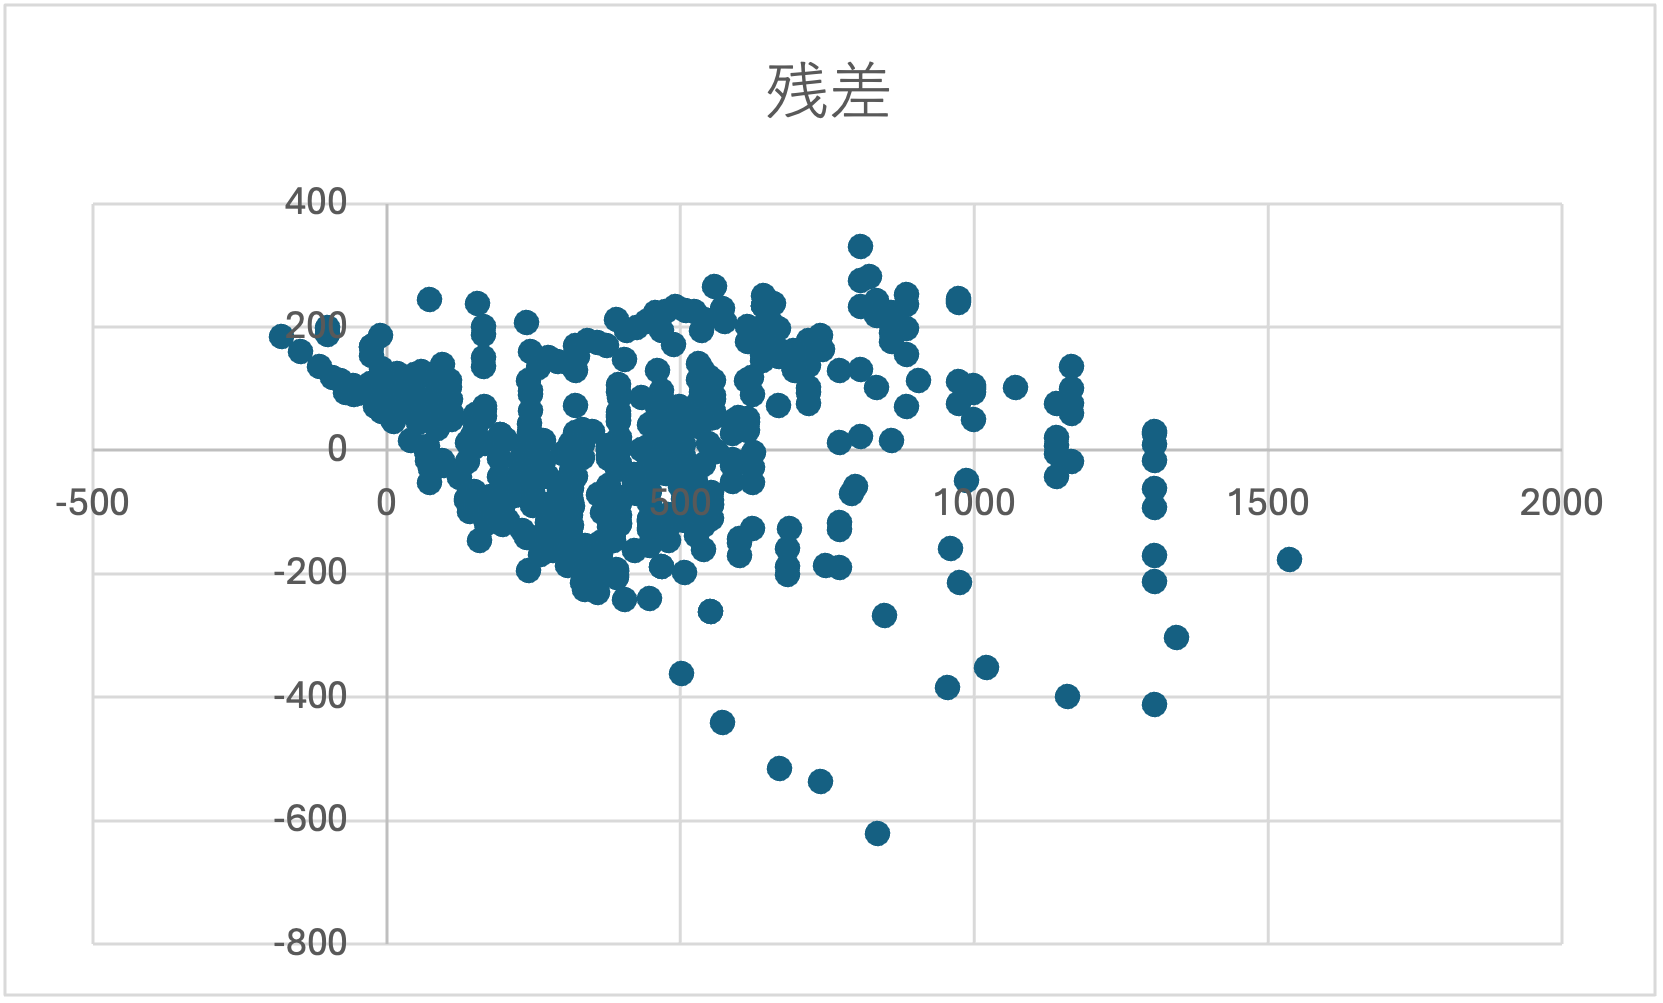
\includegraphics[width=12cm]{img/zansagraph.png}
  \caption{残差グラフ}
  \label{残差}
\end{figure}
このグラフを見るとおおよそのデータは分散しているが,一部外れ値が混ざってしまっているように見える.
おそらく,単位が正しく揃えられていないデータがあったか,ボールを質量のみで分けてしまったため,材質の違いによる違いが現れてしまったのではないかと考えられる.

重回帰積分の残差の正規性が満たされているかを確認するために正規確率プロットを描く.
描いた正規確率プロットを図\ref{正規確率}に示す.
\begin{figure}[H]
  \centering
  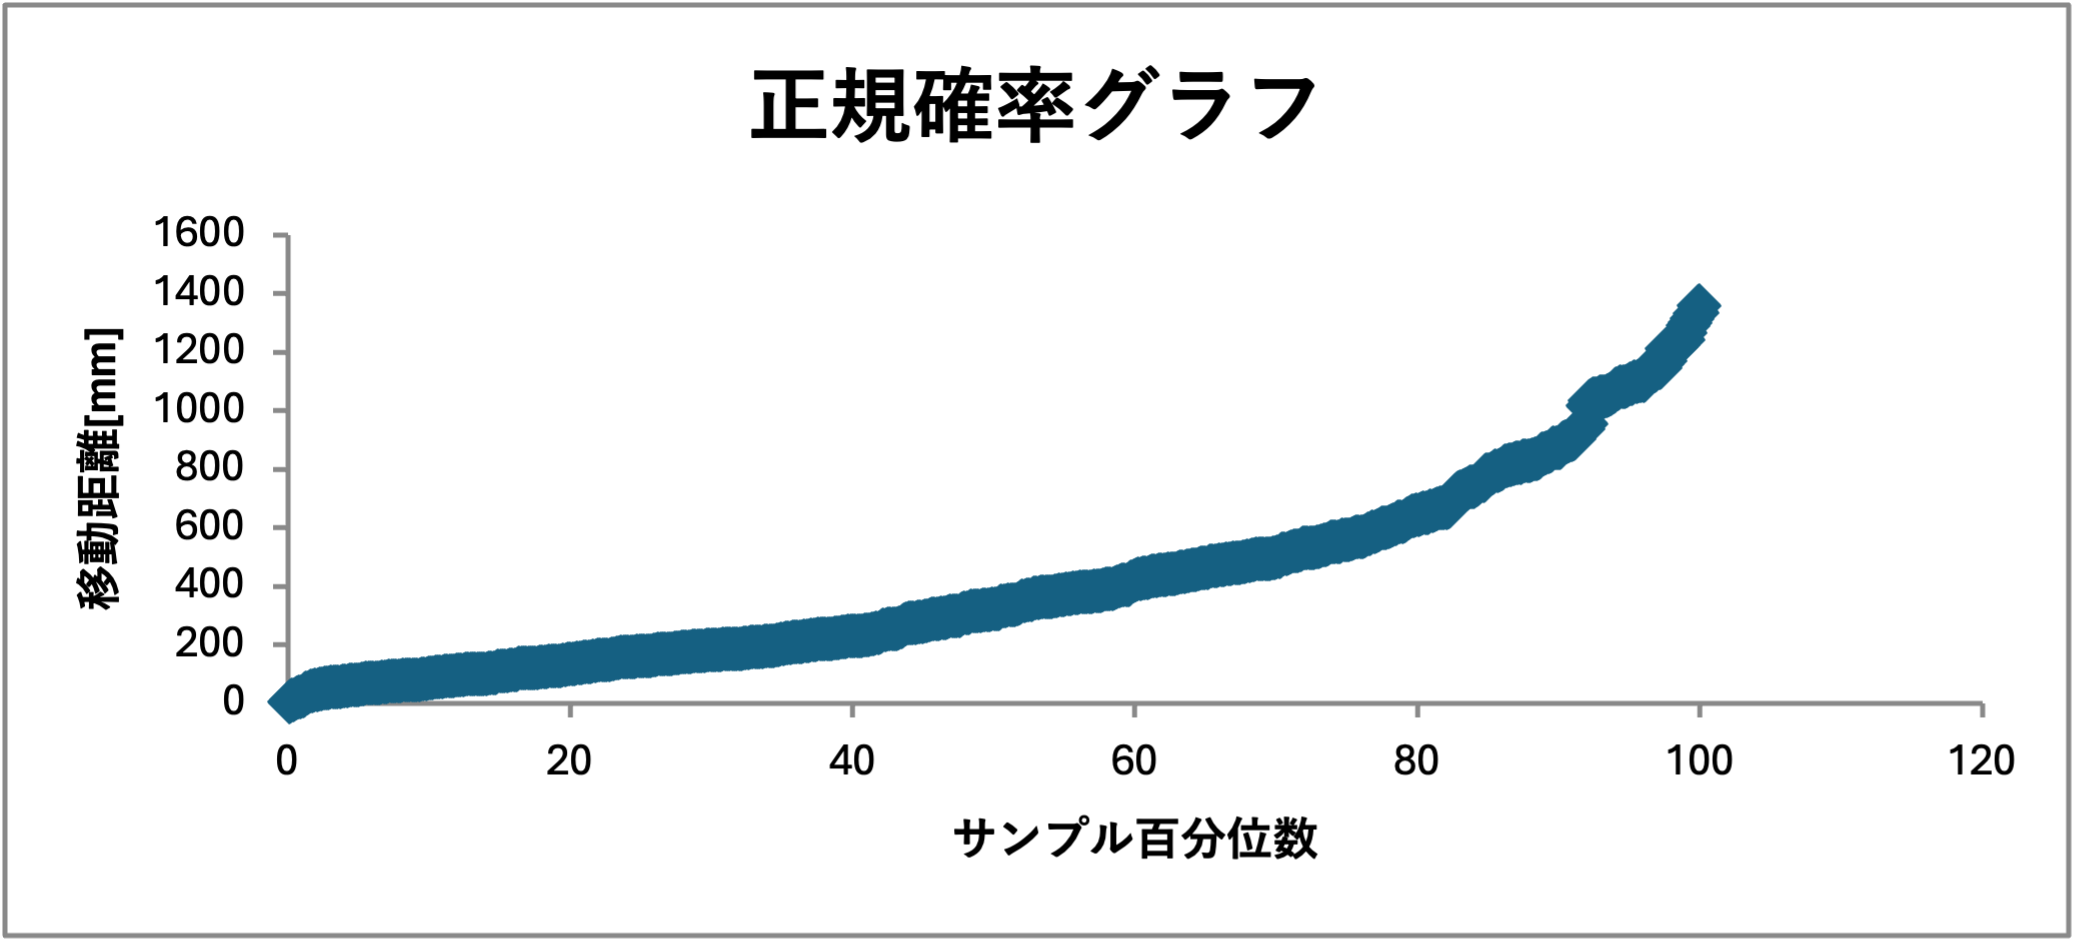
\includegraphics[width=12cm]{img/seikikakuritu.png}
  \caption{正規確率プロット}
  \label{正規確率}
\end{figure}
これを見ると,明らかに直線ではないので,目的変数である移動距離を自然対数変換する.
自然対数変換を行い,プロットし直したものを図\ref{真正規確率}に示す.
\begin{figure}[H]
  \centering
  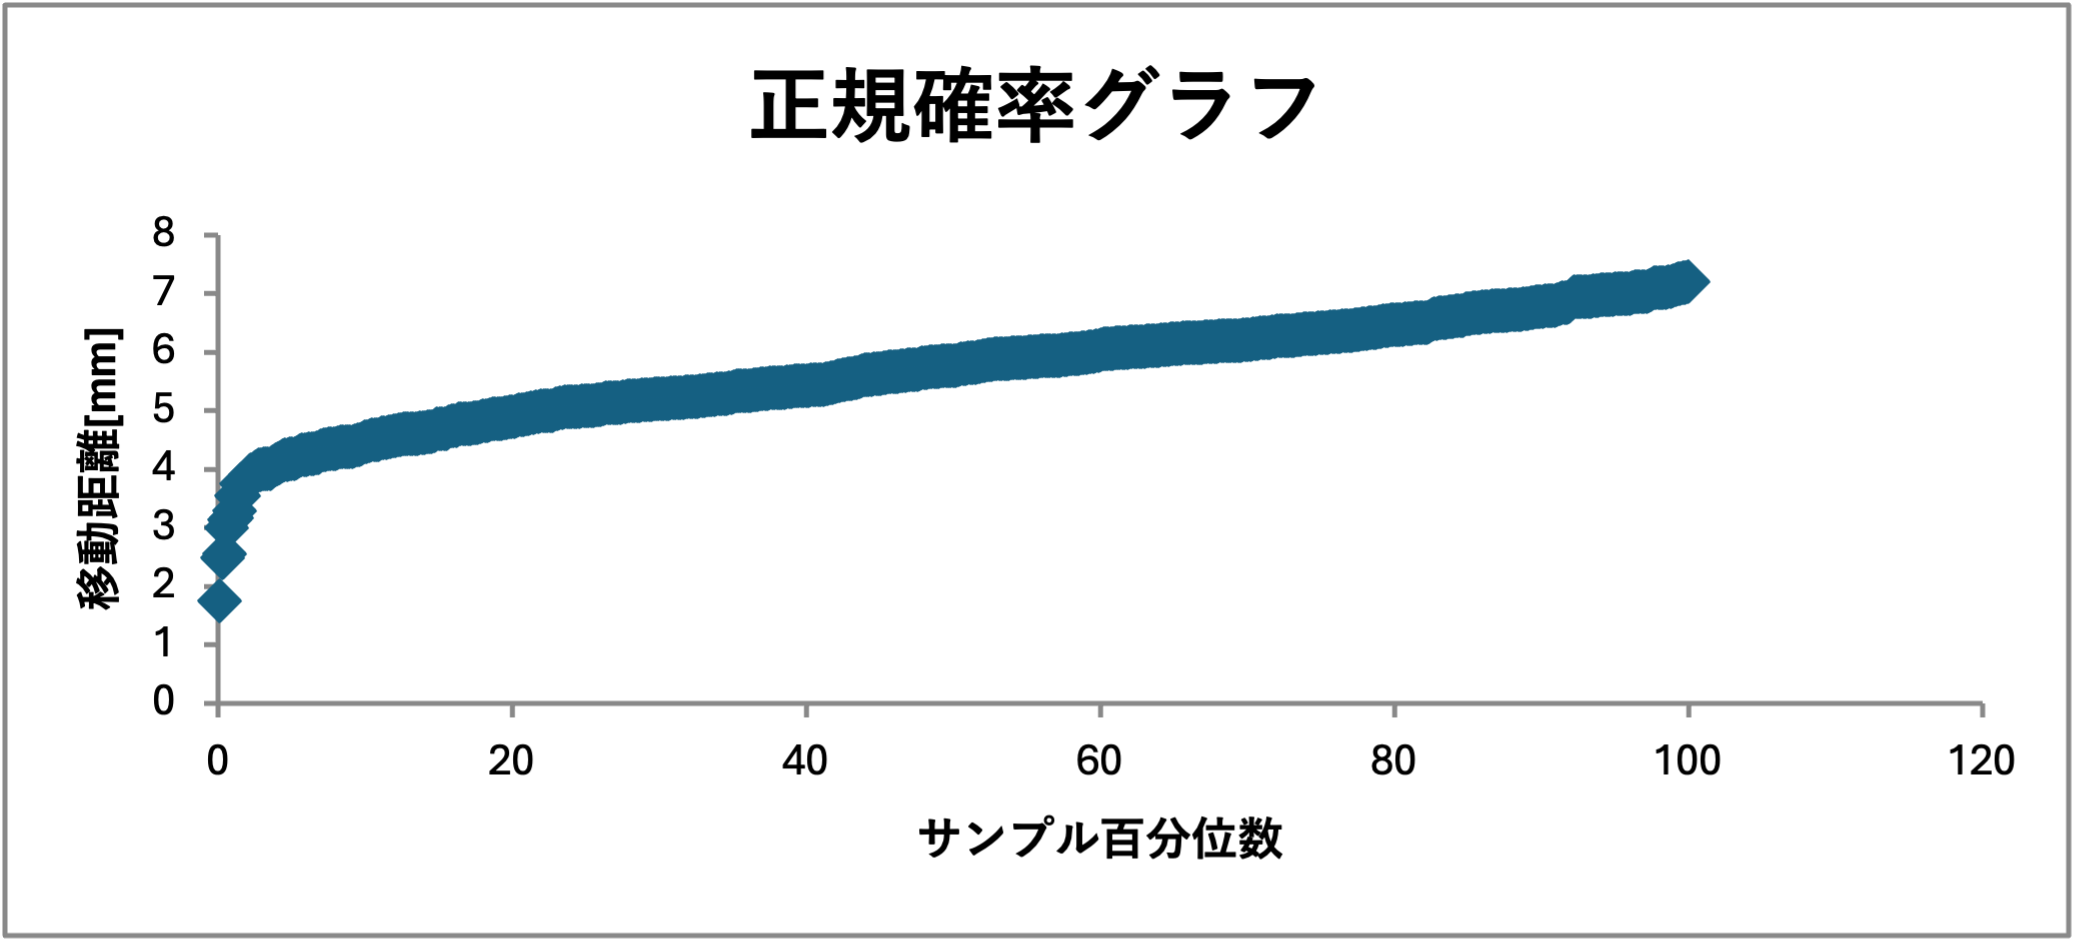
\includegraphics[width=12cm]{img/seikikakuritu_true.png}
  \caption{自然対数変換をおこなった正規確率プロット}
  \label{真正規確率}
\end{figure}
おおよそ直線であるので,式\eqref{統合重回帰式1}に示す回帰式は正規性を満たすと言える.
\section{おわりに}
\subsection{結論}
% 本分析の結論として考えられる特徴を記述
本実験では,いくつかの種類のボールを木製ブロックに衝突させ,その移動距離を測定することを通じてデータ分析の手法を学んだ.
実験データを分析する際前にデータの前処理を行い,その後相関分析や回帰分析を行うことでいくつかの説明変数が目標変数である移動距離に与える影響について分析した.

移動距離と各変数の相関関係から,高さが移動距離に最も強い相関を持つことが明らかになり,単回帰分析を用いて高さが移動距離に与える影響を具体的に定量化した.
さらに,ほかの変数も加え重回帰分析を行うことで,他の変数の影響も考慮に入れた移動距離の予測モデルを作成した.
\subsection{考察}
% 木製ブロックの移動距離に影響する要素は~等
木製ブロックの移動距離に最も影響する要素は高さと球体の質量であると考えられる.
また,それらほどではないにしろ,底辺も影響を与える事が考えられる.
\subsection{反省点}
% 反省点:球体の種類のデータ数に偏りがあった.全種類バランスよくデータを取れるように実験計画を見直す必要がある.
重回帰分析を行う際に,VIF値などを求めて最適な説明変数を探す時間がなかったため相関関係が低い変数を説明変数に用いて行ったが,
pythonやR言語などでVIF値を出力するコードを用いて,より多くの変数を用いて重回帰分析を行うべきであった.
また,統計データを扱って議論をする際にこのレポート上では不足しているデータが多々あるので,この先研究などで統計を行う際にはそのへんも解決していきたい.
\subsection{要望}
% テンプレートの統一等について,来年以降の学生に向けて欠点をお願いすること
\begin{itemize}
  \item \ref{相関:節}節の解説がなかったので,"スライドを参照すること"などでいいので多少書いてもらえると嬉しかった.
  \item データを入力する時に班によってフォーマットや基準にする単位が違い,
        全グループの統合データを作成するのがとても大変だったので,
        先生の方から表\ref{テンプレ}に示すようなテンプレートファイルを配布し,フォーマットや単位の統一を促してほしかった.
  \item iliasにレポートの提出場所を作るのが提出期限の直前になってしまっていたので実験が終わり次第すぐ上げてもらえると嬉しかった.
        また,そこにwordのテンプレートをつけてほしい.
  \item あまり期待はしていないが,TeXで書きたい学生もいるのでTeXでも対応してほしい.一応テンプレートの譲渡などできる限りの協力もできます.
  \item レポートとして重いので期末試験,期末レポートとは時期をずらしてほしい.
        もしくは授業時間をもう少し多めに取って処理をする時間を作ってほしい.
\end{itemize}
\end{document}

\begin{figure}[]
\centering
\includegraphics[width=0.8\textwidth]{}
\caption{}
\label{}
\end{figure}